\RequirePackage[l2tabu, orthodox]{nag}
\documentclass[12pt]{article}
\usepackage[utf8]{inputenc} 
\usepackage[T1]{fontenc}
\usepackage[english]{babel} 
\usepackage[margin=2.5cm]{geometry}
\geometry{a4paper}
\usepackage{longtable}


%----------------------------KODE START---------------------------------------
\usepackage{listings}
\usepackage{color}
\usepackage[usenames,dvipsnames]{xcolor}
\definecolor{gray}{rgb}{0.5,0.5,0.5}
\definecolor{mauve}{rgb}{0.58,0,0.82}
\lstset{
  basicstyle=\footnotesize,
  numbers=left,
  numberstyle=\tiny\color{gray},
  stepnumber=1,
  numbersep=10pt,
  backgroundcolor=\color{white},
  showspaces=false,               % show spaces adding particular underscores
  showstringspaces=false,         % underline spaces within strings
  showtabs=false,                 % show tabs within strings adding particular underscores
  frame=single,                   % adds a frame around the code
  rulecolor=\color{black},        
  tabsize=4,
  captionpos=b,                   % sets the caption-position to bottom
  breaklines=true,                % sets automatic line breaking
  breakatwhitespace=false,        % sets if automatic breaks should only happen at whitespace
  title=\lstname,                   % show the filename of files included with \lstinputlisting;
                                  % also try caption instead of title
  keywordstyle=\color{mauve},          % keyword style
  commentstyle=\color{Maroon},       % comment style
  stringstyle=\color{BlueViolet},         % string literal style
  escapeinside={\%*}{*)},            % if you want to add LaTeX within your code
  morekeywords={*,...},              % if you want to add more keywords to the set
  deletekeywords={...}              % if you want to delete keywords from the given language
}
%----------------------------KODE SLUT----------------------------------------


\setlength\parindent{0pt} % Makes \noindent standard
\usepackage{graphicx} 
\usepackage{caption}
\usepackage{subcaption}
\usepackage{float} 
\usepackage{wrapfig} % Allows in-line images if needed
\usepackage{hyperref}
\usepackage{amsmath}
\usepackage{amsfonts}
\usepackage{mathtools}
\hypersetup{colorlinks=false,hidelinks, citecolor=black, urlcolor=black}
\usepackage{csquotes}
\usepackage{comment}

\usepackage[dot, autosize, outputdir="dotgraphs/"]{dot2texi}
\usepackage{tikz}
\usetikzlibrary{shapes}
\usepackage{url}
\usepackage{booktabs}
\usepackage{multirow}
\usepackage{longtable}
\setcounter{secnumdepth}{4}
\setcounter{tocdepth}{4}
\usepackage[titletoc]{appendix} % Names appendices "Appendix A"
                                % instead of just A in Contents
\usepackage[bottom]{footmisc}
\usepackage{pdfpages}
\usepackage{algorithm}% http://ctan.org/pkg/algorithms
\usepackage{algpseudocode}% http://ctan.org/pkg/algorithmicx


%\usepackage{lmodern}
\usetikzlibrary{arrows,automata}
\usepackage{verbatim}

\linespread{1.2} 
\graphicspath{{./figures/}} 

% fancy drawings
\usepackage{pgf}
\usepackage{epigraph}

% \epigraphsize{\small}% Default
\setlength\epigraphwidth{8cm}
\setlength\epigraphrule{0pt}

\usepackage{etoolbox}

\makeatletter
\patchcmd{\epigraph}{\@epitext{#1}}{\itshape\@epitext{#1}}{}{}
\makeatother

%\usepackage{boxproof}
%\usepackage{nomencl}
\usepackage{natbib}

\newcommand{\fasto}{\textsc{Fasto} }
\newcommand{\mips}{\textsc{Mips} }
\newcommand{\mars}{Mars }
\makeatletter
\def\BState{\State\hskip-\ALG@thistlm}
\makeatother

%-----------------------------------------------------------------------------
\begin{document}
\begin{titlepage}

\centering 

\textsc{\Large Advanced Algorithms and Datastructures}\\[0.5cm] 
\textsc{\large Exam Notes}\\[0.5cm] 

\vfill

\emph{Author:}
\\
Jenny-Margrethe \textsc{Vej} -- 250986 -- rwj935
\vspace{20mm}

{\large Block 4, April-June, 2014}\\[3cm] 

\end{titlepage}
%-----------------------------------------------------------------------------

\tableofcontents
\newpage

%-----------------------------------------------------------------------------

\section{Maximum Flow}
Wuuuh, Max Flow!! You Rock! Kick some ass!

%\begin{quote}
%\textit{In the maximum-flow problem, we wish to compute the greatest rate at which we can ship material from the source to the sink without violating any capacity constraints.}
%\end{quote}
%%
%\subsection{Flow Networks}
%\begin{quote}
%\textit{In this section, we give a graph-theoretic definition of flow networks, discuss their properties, and define the maximum-flow problem precisely.}
%\end{quote}
%%
\subsection{Flow Networks}
\subsubsection{Flow Networks and Flow}
Let $G = (V, E)$ be a flow network with a capacity function $c$. Let $s$ be the source of the network, and let $t$ be the sink. A flow in $G$ is a real-valued function $f : V \times V \rightarrow \mathbb{R}$ that satisfies the following two properties:\\

\textbf{Capacity Constraints:} For all $u, v \in V$, we require $0 \leq f(u, v)\footnote{We call the nonnegative quantity $f(u, v)$ the flow from vertex $u$ to vertex $v$} \leq c(u, v)\footnote{Capacity Function $c$}$\\
\textbf{Flow Conservation\footnote{Vertices are conduit junctions, and other than the source and sink, material flows through the vertices without collecting in them. In other words, the rate at which material enters a vertex must equal the rate at which it leaves the vertex. This property is called Flow Conservation}:} For all $u \in V - \{s, t\}$, we require
%%
\begin{align}
\sum_{v \in V} f(v, u) = \sum_{v \in V} f(u, v)
\end{align}
%%
When $(u, v) \notin E$, there can be no flow from $u$ to $v$, and $f(u, v) = 0$. The value $|f|$ of a flow $f$ is defined as 
%%
\begin{align}
|f| = \sum_{v \in V} f(s, u) - \sum_{v \in V} f(v, s),
\end{align}

Typically, a flow network will not have any edges into the source, and the flow into the source, given by the summation $\sum_{v \in V} f(v, s)$, will be 0.
%%
\subsubsection{An example of a flow}
For example the transporting example from the book [\cite{CLRS}, p. 710]. A firm wants to transport goods from one place to anther, using a third part driver. \\

Guessing this particular section is not thaaaaat important for the exam. $\ddot\smile$

\subsubsection{Modelling problems with antiparallel edges}
Antiparallel edges is 2 edges going to/from $(v, u)$ - so 2 edges between 2 vertices but with opposite directions. To come around that, we transform our network into an equivalent one containing no antiparallel edges (adding an extra vertex for that, so we can split one of the edges). The resulting network is equivalent to the original one, due to the fact, that you do not add or subtract anything from the capacity. It is the same:\\

\begin{minipage}{.5\textwidth}
\centering
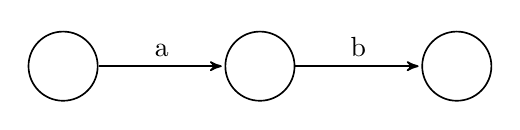
\begin{tikzpicture}[->,>=stealth',shorten >=1pt,auto,node distance=2.5cm,
                    semithick]
  \tikzstyle{every state}=[fill=none,text=black]

  \node[state] (1) {$$};
  \node[state] (2) [right of=1] {$$};
  \node[state] (3) [right of=2] {$$}; 
  
  \path 	(1)	edge node {a} (2)
  		(2)	edge node {b} (3);
\end{tikzpicture} 
\end{minipage}% 
=
\begin{minipage}{.5\textwidth}
\centering
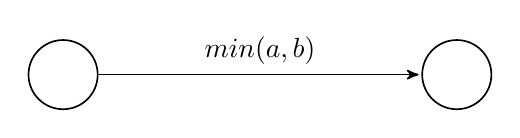
\begin{tikzpicture}[->,>=stealth',shorten >=1pt,auto,node distance=5cm,
                    semithick]
  \tikzstyle{every state}=[fill=none,text=black]

  \node[state] (1) {$$};
  \node[state] (2) [right of=1] {$$};
  
  \path 	(1)	edge node {$min(a, b)$} (2);
\end{tikzpicture} 
\end{minipage}

\subsubsection{Networks with multiple sources and sinks}
A maximum flow problem may have several sources and sinks, rather than just one of each. To fix that, we just add a supersource and a supersink with infinity capacity from $s$ to each of the multiple sources (and to $t$).
%%
\subsection{The Ford-Fulkerson Method}

\begin{algorithm}
\begin{algorithmic}[1]
\State{FORD-FULKERSON-METHOD}{$(G,s,t)$}
   \State initialise flow $f$ to $0$
   \While{there exists an augmenting path $p$ in the residual network $G_f$}
      \State augment flow $f$ along $p$
   \EndWhile
   \State \textbf{return} $f$
\end{algorithmic}
\end{algorithm}
%%
\subsubsection{Residual Network}
Suppose that we have a flow network $G = (V, E)$ with source $s$ and sink $t$. Let $f$ be a flow in $G$, and consider a pair of vertices $u, v \in V$. We define the residual capacity $c_f(u, v)$ by

\begin{align}
 c_f(u,v) =
  \begin{cases}
  	c(u,v) - f(u,v) & \text{if } (u,v) \in E, \\
  	f(v,u) & \text{if } (v,u) \in E, \\
  	0 & \text{otherwise}
  \end{cases}
\end{align}

As an example of equation (3), if $c(u, v) = 16$ and $f(u, v) = 11$, then we can increase $f(u, v)$ by up to $c_f(u, v) = 5$ units before we exceed the capacity constraint on edge $(u, v)$ We also wish to allow an algorithm to return up to 11 units of flow from $v$ to $u$, and hence $c_f(v, u) = 11$\\

Given a flow network $G = (V, E)$ and a flow $f$, the residual network of $G$ induced by $f$ is $G_f = (V, E_f)$, where
\begin{align}
	E_f = \{(u, v) \in V \cdot V : c_f(u, v) > 0\}
\end{align} 

Example:\\
\begin{minipage}{.5\textwidth}
\begin{figure}[H]
\centering
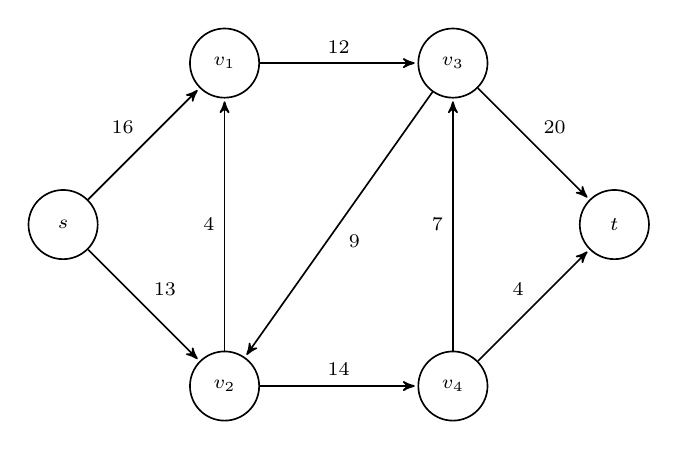
\begin{tikzpicture}[->,>=stealth',shorten >=1pt,auto,node distance=2.9cm,
                    semithick,font=\scriptsize]
  \tikzstyle{every state}=[fill=none,text=black]

  \node[state] (s) {$s$};
  \node[state] (v1) [above right of=s] {$v_1$};
  \node[state] (v2) [below right of=s] {$v_2$};
  \node[state] (v3) [right of=v1] {$v_3$};
  \node[state] (v4) [right of=v2] {$v_4$};
  \node[state] (t) [below right of=v3] {$t$};
  
  \path 	(s)	edge node {$16$} (v1)
  			edge node {$13$} (v2)
		(v1)	edge node {$12$} (v3)
		(v2)	edge node {$4$} (v1)
			edge node {$14$} (v4)
		(v3)	edge node {$9$} (v2)
			edge node {$20$} (t)
		(v4)	edge node {$7$} (v3)
			edge node {$4$} (t);
\end{tikzpicture} 
\caption{\footnotesize{Flow Network $G$}}
\end{figure}
\end{minipage}%
\begin{minipage}{.5\textwidth}
\begin{figure}[H]
\centering
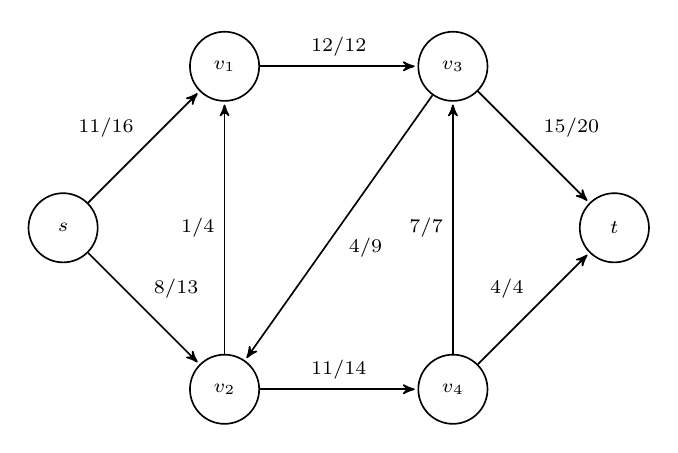
\begin{tikzpicture}[->,>=stealth',shorten >=1pt,auto,node distance=2.9cm,
                    semithick,font=\scriptsize]
  \tikzstyle{every state}=[fill=none,text=black]

  \node[state] (s) {$s$};
  \node[state] (v1) [above right of=s] {$v_1$};
  \node[state] (v2) [below right of=s] {$v_2$};
  \node[state] (v3) [right of=v1] {$v_3$};
  \node[state] (v4) [right of=v2] {$v_4$};
  \node[state] (t) [below right of=v3] {$t$};
  
  \path 	(s)	edge node {$11/16$} (v1)
  			edge node {$8/13$} (v2)
		(v1)	edge node {$12/12$} (v3)
		(v2)	edge node {$1/4$} (v1)
			edge node {$11/14$} (v4)
		(v3)	edge node {$4/9$} (v2)
			edge node {$15/20$} (t)
		(v4)	edge node {$7/7$} (v3)
			edge node {$4/4$} (t);
\end{tikzpicture} 
\caption{\footnotesize{Flow $f$ in $G$}}
\end{figure}
\end{minipage}

\begin{figure}[H]
\centering
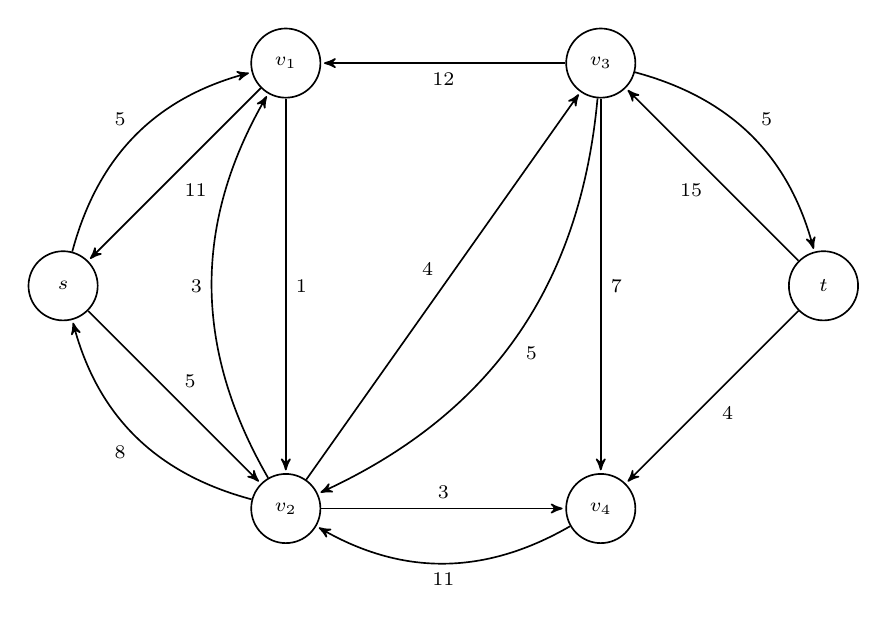
\begin{tikzpicture}[->,>=stealth',shorten >=1pt,auto,node distance=4cm,
                    semithick,font=\scriptsize]
  \tikzstyle{every state}=[fill=none,text=black]

  \node[state] (s) {$s$};
  \node[state] (v1) [above right of=s] {$v_1$};
  \node[state] (v2) [below right of=s] {$v_2$};
  \node[state] (v3) [right of=v1] {$v_3$};
  \node[state] (v4) [right of=v2] {$v_4$};
  \node[state] (t) [below right of=v3] {$t$};
  
  \path 	(s)	edge [bend left] node {$5$} (v1)
  			edge node {$5$} (v2)
		(v1)	edge node {$11$} (s)
			edge node {$1$} (v2)
		(v2)	edge [bend left] node {$3$} (v1)
			edge [bend left] node {$8$} (s)
			edge node {$4$} (v3)
			edge node {$3$} (v4)
		(v3)	edge node {$12$} (v1)
			edge [bend left] node {$5$} (v2)
			edge node {$7$} (v4)
			edge [bend left] node {$5$} (t)
		(v4)	edge [bend left] node {$11$} (v2)
		(t)	edge node {$4$} (v4)
			edge node {$15$} (v3);
\end{tikzpicture} 
\caption{\footnotesize{Residual Network $G_f$}}
\end{figure}

The residual network $G_f$ is similar to a flow network with capacities given by $c_f$. It does not satisfy the definition of a flow network because it may contain both an edge $(u, v)$ and its reversal $(v, u)$. Other than this difference, a residual network has the same properties as a flow network, and we can define a flow in the residual network as one that satisfies the definition of a flow, but with respect to capacities $c_f$ in the network $G_f$.\\

If $f$ is a flow in $G$ and $f'$ is a flow in the corresponding residual network $G_f$, we define $f \uparrow f'$, the \textbf{augmentation} of flow $f$ by $f'$, to be the function from $V \cdot V$ to $\mathbb{R}$, defined by

\begin{align}
 (f \uparrow f')(u, v) =
  \begin{cases}
  	f(u, v) + f'(u, v) - f'(v, u) \text{if } (u,v) \in E, \\
  	0 & \text{otherwise}
  \end{cases}
\end{align}

\newpage
\textbf{\textit{Lemma 26.1}}\\
Let $G = (V, E)$ be a flow network with source $s$ and sink $t$, and let $f$ be a flow in $G$. Let $G_f$ be the residual network of $G$ induced by $f$, and let $f'$ be a flow in $G_f$. Then the function $f \uparrow f'$ defined in the function (5) is a flow in $G$ with value $|$$f \uparrow f'$$|$ $=$ $|$$f$$|$ + $|$$f'$$|$.\\

\textbf{\textit{Prove for Lemma 26.1}}\\
First we check that $f \uparrow f'$ obeys capacity constraints for each edge in E and flow conservation for edges in $V-\{s, t\}$. Let us start with capacity constrains - we observe that if $(u, v) \in E$ then $c_f(v, u) = f(u, v)$. Therefore, we have $f'(v, u) \leq c_f(v, u) = f(u, v)$, and hence 
\begin{align*}
(f \uparrow f')(u, v) &= f(u, v) + f'(u, v) - f'(v, u) \qquad \text{(by equation (5))}\\
&\geq f(u, v) + f'(u, v) - f'(u, v) \qquad \text{(because} f'(v, u) \leq f(u, v))\\
&= f'(u, v)\\
&\geq 0 
\end{align*}

In addition we have, 
\begin{align*}
(f \uparrow f')(u, v) &= f(u, v) + f'(u, v) - f'(v, u) \qquad \text{(by equation (5))}\\
&\leq f(u, v) + f'(u, v) \qquad \text{(because flows are nonnegative)}\\
&\leq f(u, v) + c_f(u, v) \qquad \text{(capacity constraint)}\\
&= f(u, v) + c(u, v) - f(u, v) \qquad \text{(definition of } c_f)\\
&= c(u, v) 
\end{align*}

For flow conservation, because both $f$ and $f'$ obey flow conservation, we have that for all $u \in V - \{s, t\}$,
\begin{align*}
\sum_{v \in V} (f \uparrow f')(u, v) &= \sum_{v \in V} (f(u, v) + f'(u, v) - f'(v, u))\\
&= \sum_{v \in V} f(u, v) + \sum_{v \in V} f'(u, v) - \sum_{v \in V} f'(v, u)\\
&= \sum_{v \in V} f(v, u) + \sum_{v \in V} f'(v, u) - \sum_{v \in V} f'(u, v)\\
&= \sum_{v \in V} (f(v, u) + f'(v, u) - f'(u, v))\\
&= \sum_{v \in V} (f \uparrow f')(v, u)
\end{align*}
where the third line follows from the second by flow conservation. \\

Finally, we compute the value of $f \uparrow f'$. We remember that for any vertex $v \in V$ we can have either $(s, v)$ or $(v, s)$ but never both, because we disallow antiparallel edges in $G$. We define two sets: $V_1 = \{v : (s, v) \in E\}$ and $V_2 = \{v : (v, s) \in E\}$. Clearly $V_1$ $\cup$ $V_2 \subseteq V$ and $V_1 \cap V_2 = \emptyset$. So let us compute
\begin{align*}
| f \uparrow f' | &= \sum_{v \in V} (f \uparrow f')(s, v) - \sum_{v \in V} (f \uparrow f')(v, s)\\
&= \sum_{v \in V_1} (f \uparrow f') (s, v) - \sum_{v \in V_2} (f \uparrow f') (v, s)
\end{align*}
where the second line follows because $(f \uparrow f')(w, x)$ is $0$ if $(w, x) \notin E$. We now apply the definition of $f \uparrow f'$ to this, and then reorder and group terms to obtain
\begin{align*}
|f \uparrow f'| &= \sum_{v \in V_1}(f(s, v) - f'(v, s)) - \sum_{v \in V_2} (f(v, s) + f'(v, s))\\
&= \sum_{v \in V_1} f(s, v) + \sum_{v \in V_1} f'(s, v) - \sum_{v \in V_1} f'(v, s) - \sum_{v \in V_2} f(v, s) - \sum_{v \in V_2} f'(v, s) - \sum_{v \in V_2} f'(s, v)\\
&= \sum_{v \in V_1} f(s, v) - \sum_{v \in V_2} f(v, s) + \sum_{v \in V_1} f'(s, v) + \sum_{v \in V_2} f'(s, v) - \sum_{v \in V_1} f'(v, s) - \sum_{v \in V_2} f'(v, s)\\
&= \sum_{v \in V_1} f(s, v) - \sum_{v \in V_2} f(v, s) + \sum_{v \in V_1 \cup V_2} f'(s, v) - \sum_{v \in V_1 \cup V_2} f'(v, s)
\end{align*}
In the last line we can extend all four summations to sum over $V$, since each additional term has value $0$. Therefore we end up with 
\begin{align*}
|f \uparrow f'| &= \sum_{v \in V}(f(s, v)) - \sum_{v \in V}(f(v, s)) + \sum_{v \in V}(f'(s, v)) - \sum_{v \in V}(f'(v, s))\\
&= |f| + |f'|
\end{align*}

%
\subsubsection{Augmenting paths}
A augmenting path is a simpe path, $p$ from $s$ to $t$ in $G_f$. \\
The capacity of an augmenting path is the one of a critical edge on $p$. We can write this as $c_f(p) = min\{c_f(u, v) : (u, v) \in p\}$. The flow in $G_f$ from path $p$ can be defined as

\begin{align}
 f_p(u, v) =
  \begin{cases}
  	c_p(p) & if (u, v) \in p \\
  	0 & \text{otherwise}
  \end{cases}
\end{align}

It is now obvious that for any augmenting path $p$ we have $f \uparrow f_p$ as a flow in $G$ with $|f \uparrow f_p| = |f| + |f_p| > |f|$
%
\subsubsection{Cuts of Flow Networks}
A cut $(S, T)$, of a flow network $G = (V, E)$ is a partition of $V$ into $S$ and $T = V - S$ such that $s \in S$ and $t \in T$. We define both the flow across a cut and the capacity of a cut:

\begin{align}
f(S, T) &= \sum_{u \in S} \sum_{v \in T} f(u, v) - \sum_{u \in S} \sum_{v \in T} f(v, u)\\
c(S, T) &= \sum_{u \in S} \sum_{v \in T} c(u, v)
\end{align}

A minimum cut is a cut with minimal capacity of all cuts. \\
For any cus $(S, T)$ we have $f(S, T) = |f|$. The prove for this is:\\

First we look at the flow definition:
\begin{align*}
|f| &= \sum_{v \in V} f(s, v) - \sum_{v \in V} f(v, s)\\
&= \sum_{v \in V} f(s, v) - \sum_{v \in V} f(v, s) + \sum_{u \in S - \{s\}} \left ( \sum_{v \in V} f(u, v) - \sum_{f(v, u)}\right)
\end{align*}

Besides that, see page 722 - the main ideas is: 

\begin{enumerate}
	\item Expand the right-hand summation 
	\item Regroup into summations over $v \in V$ with edges going into $v$ and another group with edged going out of $v$
	\item Split all $v \in V$ into $v \in S$ and $v \in T$. Uses $S \cup T = V$
	\item Cancel out therms and we get what we want
\end{enumerate}

This means that $|f|$ (the value of $f$) is bounded above by the capacity of all cuts. Especially the flow is bounded above by the capacity of a minimum cut. This leeds us to the Max-flow min-cut theorem. Max-flow min-cut \textit{duality} (Pawel er fan af dette ord) is that the following are equivalent:

\begin{enumerate}
	\item $f$ is a maximum flow in $G$
	\item The residual network $G_f$ contains no augmenting paths 
	\item $|f| = c(S, T)$ for some cut $(S, T)$ of $G$
\end{enumerate}

\textbf{\textit{Proof}}\\
(1) $\Rightarrow$ (2): If we assume $f$ has a max flow, and that there is an augmenting path $p$ in $G_f$. \\
Let $f_p$ denote the max flow along $p$ - then $|f \uparrow f_p| = |f| + |f_p| > |f|$ (hence, $f \uparrow f_p$ would be a flow in $G$ wit a bigger value $\rightarrow$ contradiction)\\

(2) $\Rightarrow$ (3): We define $S = \{v \in V :$ there exists a path from $s$ to $v$ in $G_f\}$ and $T = V\setminus S (S, T)$ $\rightarrow$ is a cut. Now we would like to show $f(S, T) = c(S, T)$. \\

Consider edge $(u, v) \in E$ with $u\in S$ and $v \in T$ $\rightarrow$ $f(u, v) = c(u, v)$\\
Consider edge $(v, u) \in E$ with $u\in S$ and $v \in T$ $\rightarrow$ $f(v, u) = 0$\\

Then \begin{align*}
f(S, T) &= \sum_{u \in S, v \in T} f(u, v) - \sum_{u \in S, v \in T} f(v, u)\\
&= \sum_{u \in S, v \in T} = \sum_{u \in S, v \in T} c(u, v)\\
&= c(S, T)
\end{align*}

(3) $\Rightarrow$ (1): We let $f$ be a flow in $G$, $|f'| \leq c(S, T) = |f| \Rightarrow f$ is a max flow. (In other words - we cannot have $|f| > c(S, T)$)
%
\subsubsection{The basic Ford-Fulkerson Algorithm}
I have decided this page in the book can not be that important due to all the stuff above (The Ford-Fulkerson Algorithm is basically just an expansion on the Ford-Fulkerson Method from above)- the stuff above must be the important part (including the analysis below) for Ford-Fulkerson. But read it and remember it for the overall understanding of the topic. 
%
\subsubsection{Analysis of Ford-Fulkerson}
The running time depends on how we find the augmenting path $p$. If we assume an appropriate data structure where we can represent the directed graph, the time to find an appropriate path can be linear in the number of edges, if using breadth-first\footnote{In graph theory, breadth-first search (BFS) is a strategy for searching in a graph when search is limited to essentially two operations: (a) visit and inspect a node of a graph; (b) gain access to visit the nodes that neighbour the currently visited node. The BFS begins at a root node and inspects all the neighbouring nodes. Then for each of those neighbour nodes in turn, it inspects their neighbour nodes which were unvisited, and so on} or depth-first\footnote{Depth-first search (DFS) is an algorithm for traversing or searching tree or graph data structures. One starts at the root (selecting some arbitrary node as the root in the case of a graph) and explores as far as possible along each branch before backtracking.} search. \\

This gives os $O(E)$ work per iteration of the while loop, and at most the same number of iterations as the value of the maximum flow (since we increase by at least one unit per iteration). The total running time is therefore $O(E |f^*|)$ where $|f^*|$ is the maximum flow. 
%
\subsubsection{The Edmond-Karp Algorithm}
We can improve the bound on Ford-Fulkerson by finding the augmenting path $p$ with breadth-first search. That is, we choose the augmenting path as a shortest path from $s$ to $t$ in the residual network, where each edge has unit distance (weight). Doing this to the Ford-Fulkerson Method is called the Edmonds-Karp algorithm. \\

This gives us $O(VE^2)$ as running time. \\

First step on proving this is to see that the minimum path length (amount of edges) in $G_f$ increases monotonically. Let $\delta_f(s, v)$ be the minimum path length from $s$ to $v$ in $G_f$. Then we look at the smallest $\delta_{f'}(s, v)$ that changed when augmenting $f$ with $f'$. Let $u$ be the vertex before $v$ in the path from $s$ to $v$. We must have $\delta_{f'}(s, u) = \delta_{f'}(s, v) - 1$. We also have $\delta_f(s, u) = \delta_{f'}(s, u)$. Therefore $(u, v) \neq E_f$. We must therefore have had $\delta_f(s, v) = \delta_f(s, u) - 1$ which leads to contradiction. \\

We can use this to show that an edge can at most be critical $\frac{|V|}{2}$ times. \\

Simply look at $\delta_f(s, v) = \delta_f(s, u) +1$ when $(u, v)$ is critical. In order for the edge to return to the residual network we must have $(v, u)$ be critical. This can only happen when $\delta_{f'}(s, u) = \delta_{f'}(s, v) + 1$. Since $\delta_{f'}(s, v) + 1 \geq \delta_f(s, v) + 1 = \delta_f(s, u) +2$ the result follows. \\

Each augmenting path has at least one critical edge and only $O(VE)$ times can there be a critical edge. This gives the running time. 
%
\subsection{Maximum bipartite matching}
This topic sucks! Jeg har basically bare kopieret noter fra Søren D. Men fatter sgu ikke så meget af det. Derfor er det heller ikke med i min disposition. Håber på, jeg aldrig bliver spurgt ind til det. 

\subsubsection{The Maximum-bipartite-mathing problem}
A matching is a subset $M \subseteq E$ such that for all vertices $v \in V$ at most one edge in $M$ is incident to $v$. A maximum matching is a matching $M$ that has $|M| \geq |M'|$ for any other matching $M'$.
%
\subsubsection{Finding a maximum bipartite matching}
We can create a graph $G'$ with nodes $V' = V \cup \{s, t\}$ and edges
\begin{align*}
E' = \{(s, u) : u \in L\} \cup \{(u, v) : (u, v) \in E \} \cup \{(u, t) : u \in R\}
\end{align*}

All capacities $c(u, v) = 1$. It is clear that $|E'| = O(|E|)$ because we assume each node $v \in L \cup R$ has one edge incident in $E$. \\

We wanna show that a flow $f$ in $G'$ corresponds to a matching $M$ in $G$. First we say that a flow is integer-valued if $f(u,v)$ is integer for all $(u,v) \in V 	\cdot V$. The claim is that if $M$ is a matching in $G$ it corresponds to a flow $f$ in $G'$ with $|f| = |M|$ and the other way around.\\

To proof this, we say for a matching $M$ create a flow $f(u, v) = f(s, u) = f(u, t) = 1$ for all $(u, v) \in M$. It is easy to see that the constraints are satisfied and that $|f| = |M|$. For a flow $f$ we create a matching
\begin{align*}
	M = \{(u, v) : u \in L, v \in R, \text{and} f(u, v) > 0 
\end{align*}
Because $f$ is integer-valued this is okay. To see that this is a matching use that $(s, u) = 1$ and flow conservation means the sum over $(u, v) = 1$ (or $0$). We can also use this to show that $|M| = |f|$. \\

We also need to show that when $c(u, v)$ is integral for all $(u, v)$ the maximum flow found by Ford-Fulkerson will be integer-valued. This is done easily by induction over the iteration. Base case is trivial cause $|f| = 0$.\\

We can now proof by contradiction that a maximum flow corresponds to a maximum matching.

\subsection{Disposition}
\newpage

\section{Fibonacci Heaps}
Okaaaaaay! This is awesome! Kick some serious ass!

\subsection{Structure of Fibonacci Heaps}
A Fibonacci Heap is a collection of rooted trees that are min-heap ordered. That is, each tree obeys the min-heap property: the key of a node is greater than or equal to the key of its parent. 

\begin{figure} [H]
    \begin{center}
        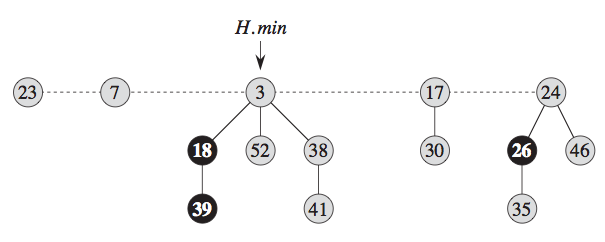
\includegraphics[width=\textwidth]{Images/Hmin.png}
        \caption{Fibonacci heap consisting of five min-heap-ordered trees and 14 nodes}
        \label{fig:H.min}
    \end{center}
\end{figure}



\subsubsection{Potential Function}
\subsubsection{Maximum Degree}

\subsection{Mergeable-heap Operations}
\subsubsection{Creating a New Fibonacci Heap}
\subsubsection{Inserting a Node}
\subsubsection{Finding the Minimum Node}
\subsubsection{Uniting Two Fibonacci Heaps}
\subsubsection{Extracting the Minimum Node}

\subsection{Decreasing a Key and Deleting a Node}
\subsubsection{Decreasing a Key}
\subsubsection{Deleting a Node}

\subsection{Bounding the Maximum Degree}

\subsection{Disposition}
\newpage

\section{NP-Completeness}
\newpage

\section{Randomised Algorithms}
\newpage

\section{Hashing}
OMG LOLZ'n SHIZZLES! You'r gonna nail this shit!

\subsection{Direct-address tables}
We have a scenario where we want to maintain a dynamic set of some sort. Each element has a key drawn from a universe $U = \{0, 1, ..., m-1\}$ where $m$ is not too large, and no two elements have the same key. \\

Representing it by a direct-address table, or array $T[0...m-1]$, each slot or position corresponds to a key  in $U$. If there is an element $x$ with the key $k$, then $T[k]$ contains a pointer to $x$ - otherwise $T[k]$ is empty represented by $NIL$\\

Illustration in the book on page 254
\begin{algorithm}
\begin{algorithmic}[1]
\State{DIRECT-ADDRESS-SEARCH}{$(T, k)$}
   \State \textbf{return} $T[k]$\\
   
\State{DIRECT-ADDRESS-INSERT}{$T, x$}
   \State \textbf{return} $T[key[x]] \leftarrow x$\\

\State{DIRECT-ADDRESS-DELETE}{$T, x$}
   \State \textbf{return} $T[key[x]] \leftarrow NIL$
\end{algorithmic}
\end{algorithm}

Downsides of direct addressing: If the universe $U$ is large, storing a table $T$ of size $|U|$ may be impractical or even impossible, given the memory available on a typical computer. Furthermore, the set $K$ of keys actually stored may be so small relative to $U$ that most of the space allocated for $T$ would be wasted. 

\subsection{Hash tables}
To overcome the downsides of direct addressing, we can use hash tables. When $K$ is much smaller than $U$, a hash table requires much less space than a direct-address table. It can also reduce storage requirements to $\Theta (|K|)$. \\

This bound is for average-case time whereas for direct addressing it holds for the worst-case time. \\

With direct addressing, an element with $k$ is stored in slot $k$. With hashing, this element is stores in slot $h(k)$; that is, we use a hash function $h$ to compute the slot from the key $k$. There is one hitch: 2 keys may hash to the same slot - called a collision. See page 256 for illustrations. \\

A hash function $h$ must be deterministic in that a given input $k$ should always produce the same output $h(k)$. \\

\textbf{Collision resolution by chaining}\\
In chaining we place all the elements that hash to the same slot into the same linked list. See figure on page 257.

\begin{algorithm}
\begin{algorithmic}[1]
\State{DIRECT-HASH-SEARCH}{$(T, x)$}
   \State \textbf{search} for an element with key $k$ in list $T(T, k)$\\
   
\State{DIRECT-HASH-INSERT}{$T, x$}
   \State \textbf{insert} $x$ at the head of the list $T[h(x.key)]$\\

\State{DIRECT-HASH-DELETE}{$T, x$}
   \State \textbf{delete} $x$ from the list $T[h(x.key)]$
\end{algorithmic}
\end{algorithm}

\textbf{Analysis of hashing with chaining}\\
Given a hash table $T$ with $m$ slots that stores $n$ elements, we define the load factor $\alpha$ for $T$ as $n/m$ which is the same as the average number of elements stores in a chain. \\

Worst case performing: $\Theta (n)$ + the time to compute the hash function (all $n$ keys hash to the same slot, creating a list of length $n$. \\

Average case performing of hashing depends on how well the hash function $h$ distributes the set of keys to be stores among the $m$ slots, on the average. \\

\textbf{\textit{Theorem 11.1}}
In a hash table in which collisions are resolved by chaining, an unsuccessful search takes an average-case time $\Theta (1 + \alpha)$, under the assumption of simple uniform hashing. (OBS: Beviset herfor står på side 259!! LÆS OG FORSTÅ)\\

\textbf{\textit{Theorem 11.2}} 
In a hash table in which collisions are resolved by chaining, a successful search takes average-case time $\Theta (1 + \alpha)$, under the assumption of simple uniform hashing. (OBS: Beviset herfor står på side 259-260!! LÆS OG FORSTÅ)

\subsection{Hash functions}
\textbf{What makes a good hash function?} \\
A good hash function satisfies (approximately) the assumption of simple uniform hashing: each key is equally likely to hash to any of the $m$ slots, independently of where any other key has hashed to. In practice, we can often employ heuristic techniques to create a hash function that performs well. \\

\textbf{Interpreting keys as natural numbers}\\
Most hash functions assume that the universe of keys is the set $\mathbb{N} = \{0, 1, 2, ...\}$ of natural numbers. 

\subsubsection{The division method}
\subsubsection{The multiplication method}
\subsubsection{Universal hashing}
\subsection{Open addressing}
\subsection{Perfect hashing}
\newpage

\section{Exact Exponential Algorithms}
\newpage

\section{Approximation Algorithms}
\newpage

\section{Computational Geometry}
\newpage

\section{Linear Programming and Optimisation}
[\cite{monoids}]

\newpage
\bibliographystyle{plainnat}
%\bibliographystyle{unsrt}
\bibliography{bibliography}


%-----------------------------------------------------------------------------
\end{document}